\section{Continuity}
We have seen several theorems showing that limits ``behave nicely" when we mix them with other operations. All these results are variations on the same theme; when $a_n, b_n$ get close to their limits $\alpha, \beta$, then $a_n+b_n$ is close to $\alpha+\beta$, $a_nb_n$ is close to $\alpha\beta$ and so on. We have not said much about trig functions or logarithms; we expect that the reader has some familiarity with such things, but it takes a fair amount of work just to get a completely precise definition of what these functions are, so we have put them aside for the moment. Nevertheless it makes sense to expect that, when $n$ is large enough, $\sin(a_n)$ will be close to $\sin(\alpha)$ et cetera. This is the way we expect most functions to behave, and it is essential for most uses of mathematics to describe the world, since all measurements are inexact. When we measure the angle between two laser beams or two metal bars, the most we can say that is very close to 47 degrees; we could not make much use of trigonometry  in engineering without some guarantee that the sine of this angle must be close to $\sin(47^\circ)$. We encapsulate this idea with the following (preliminary) definition:

\begin{defn}\label{def:continuityPrelim}
The function $f$ is \emph{continuous} at $\alpha$ if
\[\lim f(a_n) = f(\alpha)\]
for all convergent sequences with $\lim a_n = \alpha$.
\end{defn}

This definition will need a bit of tweaking, but before delving into the technical details one should make sure  to understand that this formal definition sums up the intuitive ideas of the preceding paragraph. Note that we have already implicitly proved a result along the lines of ``most normal-looking functions are continuous":

\begin{thm}\label{thm:ratFunctsCont}
Let $f(x)=\frac{p(x)}{q(x)}$ where $p,q$ are polynomials. Then $f$ is continuous everywhere it is defined (i.e. everywhere that $q(x) \neq 0$).

A function of this form is called a  \emph{rational} function.
\end{thm}
\begin{proof}
Let $p(x) = p_nx^n + \cdots + p_1x + p_0$ and $q(x) = q_mx^m + \cdots + q_1x + q_0$.
Our previous results on sums and products tell us that, if $a_n$ converges to $\alpha$,
\[
\lim p(a_n) = p_n(\lim a_n)^n + \cdots + p_1(\lim a_n) + p_0 = p(\alpha)
\]
and
\[
\lim q(a_n) = q_m(\lim a_n)^m + \cdots + q_1(\lim a_n) + q_0 = q(\alpha)
\]
Since the limits exist, we also already know that, if $q(\alpha)\neq0$, 
\[
\lim f(a_n)=\frac{\lim p(a_n)}{\lim q(a_n)}=f(\alpha)
\]
\end{proof}

The proof of  (\ref{thm:ratFunctsCont}) points toward the tweaks we need. In order for the definition to make any sense, our  $f$ must be defined at $\alpha$; furthermore the only sequences that make sense here are those with values in the domain of $f$, so that each $f(a_n)$ is defined. In fact, we are going to restrict things even more. We are interested in what happens to $f(x)$ as $x$ gets close to $\alpha$, so we want $f$ to be defined at all points ``around" $\alpha$; in other words, $f$ should be defined on an \emph{open interval} containing alpha, leading to

\begin{defn}\label{def:continuity}
The function $f$ is \emph{continuous} at $\alpha$ if it is defined at all points in an open interval $I$ containing $\alpha$ and 
\[\lim f(a_n) = f(\alpha)\]
for all convergent sequences $a_n$ with values in I and $\lim a_n = \alpha$.
\end{defn}
Note that this definition implicitly requires that $f(a_n)$ must be convergent for all such $a_n$. Recall that an open interval $(a,b)$ is the set of all $x$ such that $a < x < b$; since we exclude the endpoints, our interval $I$ must contain points on both sides of $\alpha$.

Recall theorem \ref{thm:subsequenceLim}, which states that $\lim a_n = \alpha$ is determined by any tail subsequence $a_k, a_{k+1} \cdots$. If $I$ is an open interval and $\lim a_n \in I$, We will have $a_n \in I$ when $n$ is large enough (take $\varepsilon$ small enough to get $(\alpha-\varepsilon,\alpha+\varepsilon)$ inside $I$). This means that any convergent sequence approaching $\alpha$ is applicable to the definition of continuity, if we truncate it enough to keep only values that are within the domain of $f$.

Our theorems about the behavior of limits under various operations carry over directly to continuous functions, for instance

\begin{thm}\label{thm:sumOfCont}
If functions $f,g$ are continuous at $\alpha$ then so is $f+g$.
\end{thm}
\begin{proof} Follows almost immediately from results on sequences. \end{proof}

\subsubsection{Exercises}
\begin{itemize}
\item Prove the claim made above that there is a tail of $\{a_n\}$ contained in $I$.
\item Composition, product of continuous functions are continuous. Absolute value is continuous.
\end{itemize}


\subsection{Graphs of Continuous Functions}
Continuity is closely related to our expectation of what the graph of a function should look like. The functions studied in precalculus -- polynomials, trig, square roots et cetera -- have graphs that can be drawn as smooth unbroken curves, ``without lifting the pen from the paper" (in the classic phrase of the pre-computer era); the only exceptions are the few points where these functions are undefined, such as $\frac{1}{x}$ at $x=0$. A function whose graph has a visual break is discontinuous at that point even if it is defined there. A good example is the ceiling function $\lceil x \rceil$ introduced in the last chapter. It is discontinuous at every integer; for instance $\lceil 1 \rceil = 1$, but $\lim \lceil 1 + \frac{1}{n} \rceil = 2$.
%For instance the ``sign" (not sine!) function (see figure \ref{fig:discontinuity})
%\[
%f(x) = \begin{cases}
%1, &x > 0\\
%0, &x = 0\\
%-1, &x < 0
%\end{cases}
%\]
%is discontinuous at zero; any sequence of positive numbers with $\lim a_n = 0$ will have $\lim f(a_n) = 1$. Note that it would be discontinuous no matter how we defined $f(0)$.

A more extreme example would be
\[
f(x) = \begin{cases}
1, &x\  \text{is rational}\\
0, &x\  \text{is irrational}
\end{cases}
\]
which jumps around so much that it cannot be drawn as a curve at all; it is discontinuous everywhere (see exercise ??). 

The most ``well-behaved" functions should be ones that could plausibly represent the motion of a physical object; assuming objects cannot teleport, such motion defines an unbroken curve. Similar considerations apply to other physical quantities: temperature cannot rise from $99$ to $100$ degrees without momentarily passing through each intermediate $99 < y < 100$ et cetera. The definition of continuity is an attempt to capture some of that intuition. We will see in section \ref{sec:behaviorOfContFuncs} that continuous functions can still behave in physically implausible ways, but first we will consider the consequences of this ``intermediate value" property, which, stated more precisely, claims:

\begin{claim}[The Intermediate Value Property]\label{claim:intermediateValue}
Let $f$ be continuous at all points of the closed interval $[a,b]$, with $f(a)<f(b)$. Then for any $f(a) < y' < f(b)$ there exists $a < x' < b$ such that $f(x') = y'$.
\end{claim}
This assertion is bolder than it might appear. Consider $f(x)=x^2$ on the interval $[1,2]$; we are claiming that $x^2$ will take every value from 1 through 4. In particular we must somewhere have $f(x') = 2$. But that can only mean $x' = \sqrt{2}$. We have already noted that there is no absolute reason why there must be a square root of 2; in the logically consistent world that has no irrational numbers, the claim is false! Putting it the other way around, the claim cannot be proved without using our promised assumption about the fullness of the real numbers, so is time to state that assumption precisely. The preliminary version asserted that all decimal expansions specify numbers; a more useful expression of the same idea uses the following 

\begin{defn}
A sequence $\{a_n\}$ is called a \emph{Cauchy sequence}\footnote{After the French mathematician Augustin-Louis Cauchy, 1789-1857; approximated in English as ``co-shee"} if, given any $\varepsilon > 0$, there is an $N_\varepsilon$ for which
\[
|a_n - a_m| < \varepsilon
\]
whenever $n,m$ are \emph{both} greater than $N_\varepsilon$.
\end{defn}

With this definition, we make the following

\begin{assumption}
All Cauchy sequences converge
\end{assumption}

The intuition here is identical to our earlier heuristic argument about decimals: if we imagine plotting a dot on the line for each term of $\{a_n\}$, these dots will be confined within smaller and smaller segments nested within one another, and the limit is the one point which is inside all segments. In figure \ref{fig:cauchy}, the entire tail sequence $a_{n_1}, a_{n_1+1}, \cdots$ is contained in the open interval $(a_{n_1}-\varepsilon, a_{n_1}+\varepsilon)$; taking some $n_2>n_1$ and a small enough $\varepsilon_2$, we can get an open interval around $a_{n_2}$, contained within the first interval, which holds all of $a_{n_2}, a_{n_2+1} \cdots$, and may continue with ever-smaller intervals.

The property of all Cauchy sequences being convergent is called \emph{completeness}.

\begin{figure}
\begin{center}
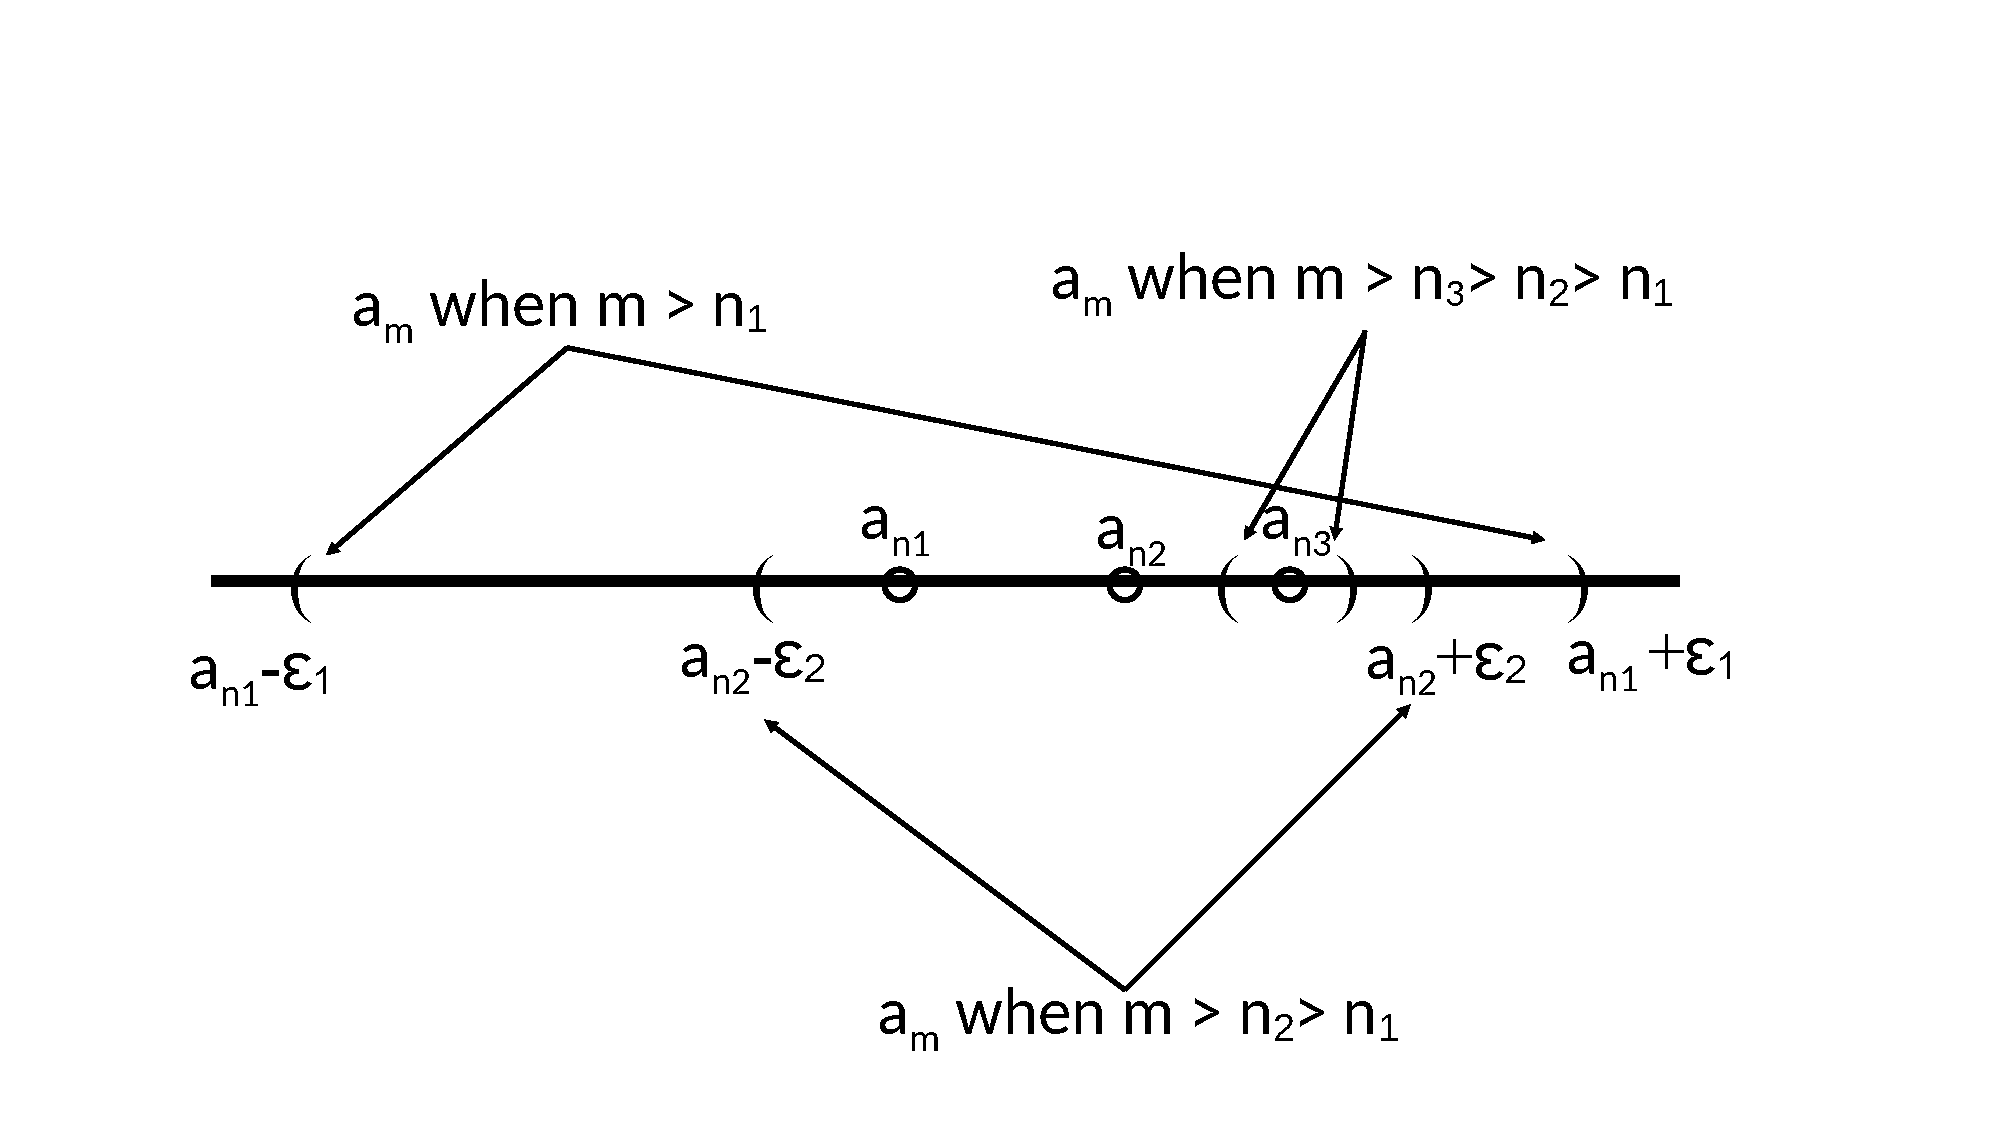
\includegraphics[scale=0.25]{cauchy}
\end{center}
\caption{Convergence of a Cauchy Sequence \label{fig:cauchy}}
\end{figure}

\subsubsection{Exercises}
\begin{itemize}
\item Suppose $f$ is allowed to be non-continuous at just one point in $[a,b]$; can we still guarantee the existence of $a < x' < b$ such that $f(x') = y'$?
\item Prove that every convergent sequence is a Cauchy sequence; this is true with or without our assumption.
\item Prove that every decimal expansion converges -- i.e., as promised, every infinite series of the form
\begin{equation}\label{eq:decimalExpansionExercise}
\sum \frac{d_n}{10^n}
\end{equation}
 (where each $d_n$ is a digit, i.e. an integer in the range 0 to 9) converges.
\item Let $\lim a_n = \alpha$. Prove that $\alpha$ can be represented by a decimal expansion -- i.e. there is a series of the above form which converges to $\alpha$.
\end{itemize}


\subsection{The Intermediate Value Theorem}
We now prove that the convergence of Cauchy sequences -- i.e. the completeness of the real numbers --``fills up" the number line enough to yield the intermediate value property. Let $a,b,f,y'$ be as in claim (\ref{claim:intermediateValue}). Given the tools at our disposal, there is only one thing to try to do: find a Cauchy sequence $\{x_i\}$ such that $\lim f(x_i) = y'$. Then completeness means that $\{x_i\}$ converges to a real number $x'$, and continuity implies $f(x')=y'$.

Geometric intuition tells us that that somewhere the graph of $f$ must cross over the horizontal line $y=y'$, so our strategy is to narrow down where this happens.  We begin by dividing the problem in half, letting $x_0=a, x_1=b$ and $x_2 = \frac{a+b}{2}$. There is nothing more to prove if $f(x_2)=y'$, otherwise we continue with
\[
x_3 = 
\begin{cases}
a+\frac{b-a}{4}, &\text{if $f(x_2)<y'$}\\
a+3\frac{b-a}{4}, &\text{if $f(x_2)>y'$}\\
\end{cases}
\]
i.e we go halfway toward one endpoint or the other, in whatever direction will put the crossover point between $x_2$ and $x_3$. We continue in this manner (see figure \ref{fig:IVP}); after selecting $x_j$ we limit our attention to an interval of width $\frac{b-a}{2^j}$, which is either $(x_i,x_j)$ with $f(x_i) < y < f(x_j)$ or $(x_j,x_i)$ with $f(x_j) < y < f(x_i)$ (for some $i<j$); then $x_{j+1}$ will be the midpoint of this interval.

We can stop if we ever get $f(x_j)=y'$: otherwise the $\{x_i\}$ are a Cauchy sequence, because the tail $x_j, x_{j+i} \cdots$ is contained within an interval of width $\frac{b-a}{2^j}$. We claim its limit is the required $x'$. Consider two subsequences of $\{x_i\}$: one consisting of all $x_k$ with $f(x_k) < y'$, call this sequence $\{x^{-}_i\}$, and the other terms  $\{x^{+}_i\}$. If both of these subsequences are infinite, they both converge to $x'$. Now the sequence $f(x^{-}_i)$ has all terms less than $y'$, so its limit, which is $f(x')$, must be less than or equal to $y'$; similarly $f(x')=\lim f(x^{+}_i) \geq y'$, so $f(x')=y$.

\begin{figure}
\begin{center}
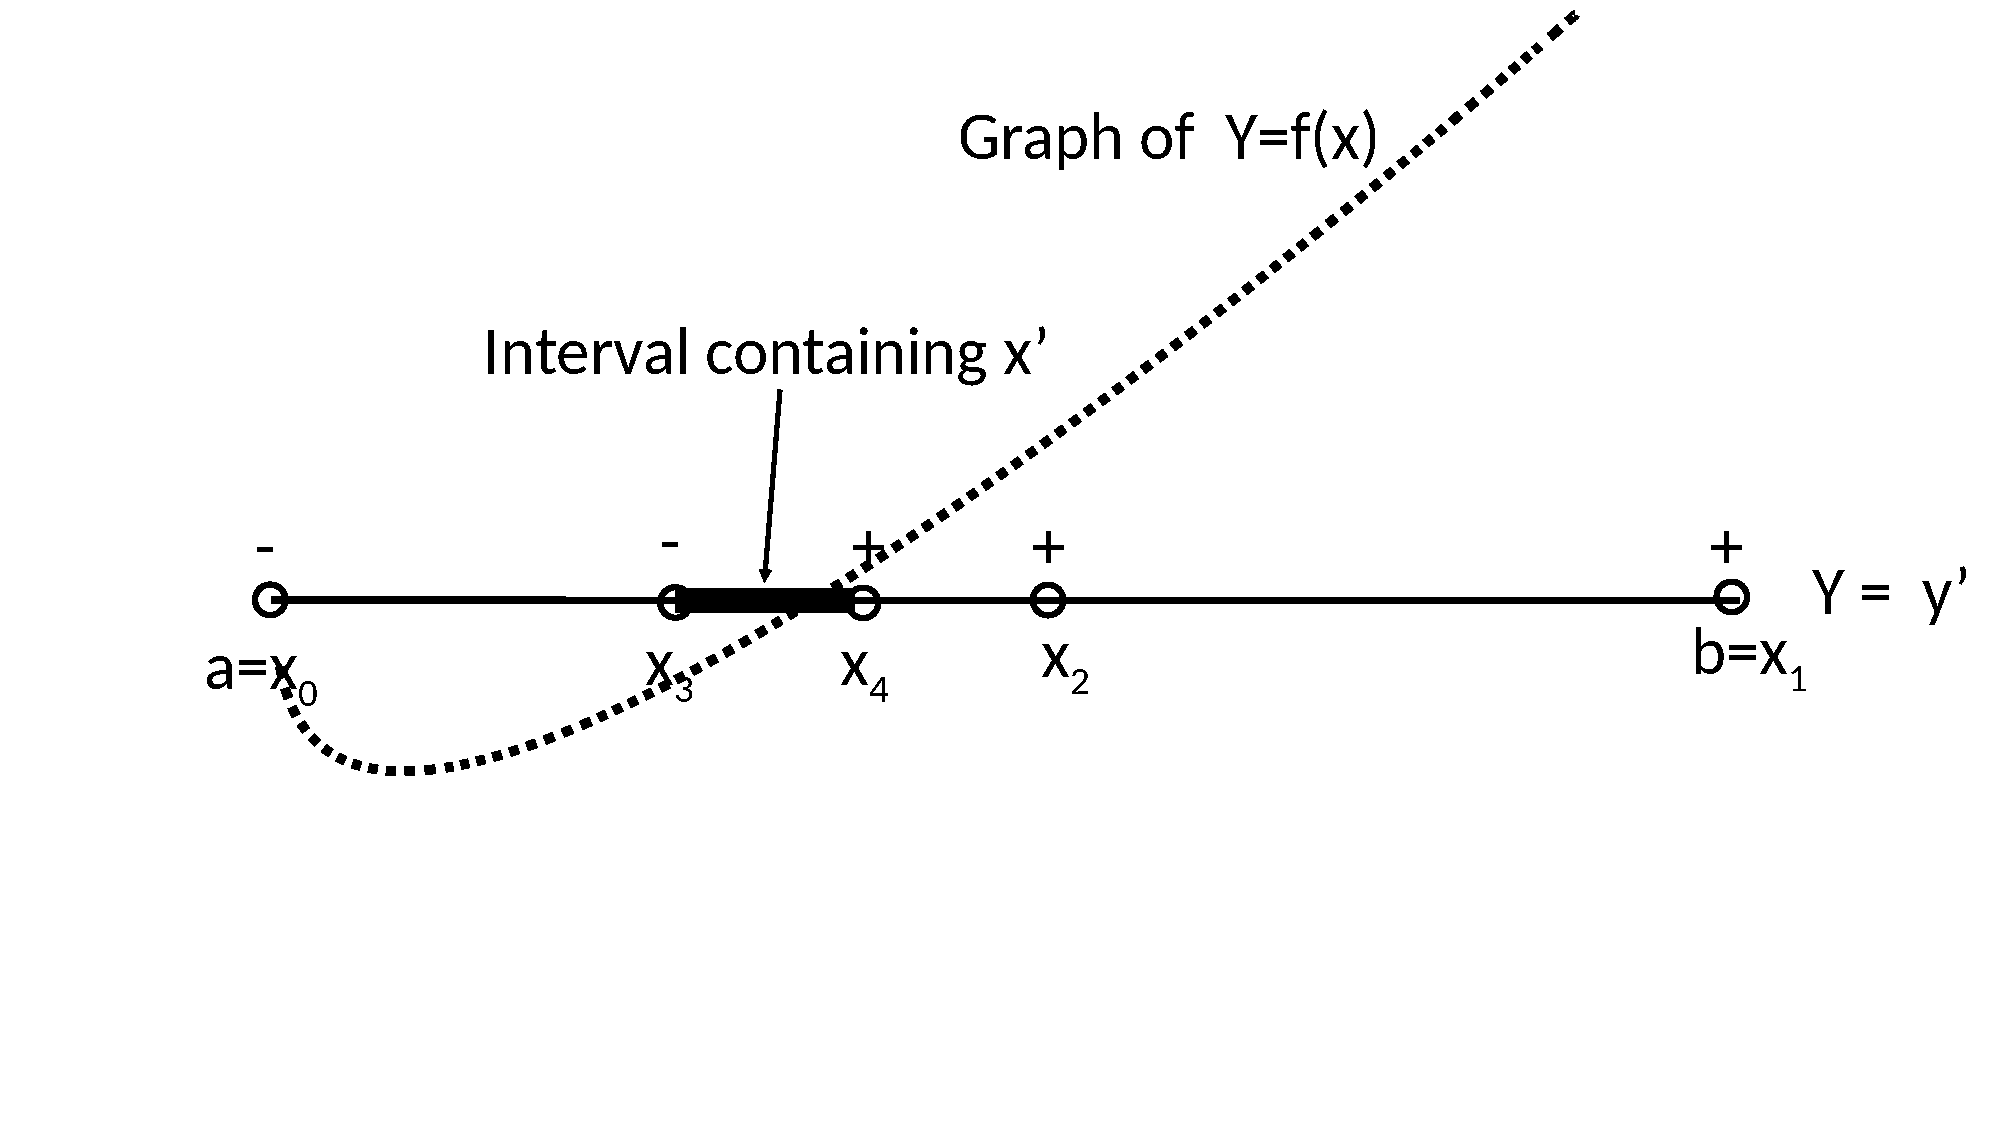
\includegraphics[scale=0.25]{IVP}
\end{center}
\caption{Proof of the Intermediate Value Property \label{fig:IVP}}
\end{figure}


Finally we must dispense with the possibility that one of these subsequences, say $\{x^{+}_i\}$, is finite. In that case there must be a largest index $M$ at which $f(x_M)>y'$. From the definition of the sequence we would necessarily have $x_i = M - \frac{b-a}{2^i}$ for every $i>M$. But that is impossible: we would get $x' = \lim x_i = x_M$ and thus $\lim f(x_i) = f(x_M) > y'$ while every $f(x_i) < y'$.

%It is a useful definition because it captures what makes a sequence convergent without making any explicit reference to the limit; if we deny the existence of irrationals it makes no difference, a Cauchy sequence is still a Cauchy sequence.

{\color{red}
\subsubsection{Exercises}
Least upper bounds; maximum/minimum  of continuous function on a closed interval.
%Need intermediate value for chain rule? inverse functions?
}

\subsection{Behavior of Continuous Functions}\label{sec:behaviorOfContFuncs}
This section is optional, i.e. subsequent material does not depend on it. Since it is optional we will cheat a bit and make use of the sine function even though we have not formally defined it. We know that its graph crosses the $x$-axis infinitely often, at each $x_0=k\pi$. Thus the graph of $f(x) = \sin(1/x)$ looks like figure ??; in any open interval around zero it changes direction and crosses the $x$-axis infinitely many times. It will be discontinuous at zero no matter what value we assign to $f(0)$; different sequences $a_n$ with $\lim a_n = 0$ could have $\lim f(a_n)$ equal to any $-1 \leq \alpha \leq 1$, or the limit might not exist (exercise: give examples of such). But we can tame this wildness somewhat by defining
\[
g(x) = \begin{cases}
|x|\sin(1/x), &x \neq 0\\
0, &x = 0
\end{cases}
\]
to get something that looks like figure ??. Now the infinite fluctuations keep getting smaller, and $\lim a_n = 0$ does imply $\lim f(a_n) = 0$ because $|f(a_n)| \leq |a_n|$ (exercise: finish the proof). Thus $g$ is continuous everywhere. Yet we still cannot imagine drawing the entire graph, and we doubt that any object could move this way, as it would require infinitely many changes of direction in a finite space and time.

\subsubsection{Exercises}
Anything else?

%\subsection{Limit of a function at a point}
%Whether or not a function $f$ is continuous at $\alpha$, we define
%
%\begin{defn}
%Let $f$ be defined at all points on an open interval $I$ containing $\alpha$, except perhaps $\alpha$ itself. If there is a $\beta$ such that
%\[\lim f(a_n) = \beta\]
%for all convergent sequences $a_n$ with values in $I\setminus\{\alpha\}$\footnote{This is the notation for the \emph{difference} of two sets: $A \setminus B$ consists of all elements of $A$ that are not in $B$. Here it says we remove the single point $\alpha$ from $I$.}
%and $\lim a_n = \alpha$, we write
%\[\lim_{x \to \alpha} f(x) = \beta\]
%and call $\beta$ the limit of $f$ at $\alpha$.
%\end{defn}
%
%We can apply this definition to something like
%\[
%g(x) = \begin{cases}
%1, &x \neq 0\\
%0, &x = 0
%\end{cases}
%\]
%which is discontinuous at zero but has $\lim_{x\to0} g(x) = 1$; note that it is essential in the definition to exclude $\alpha$, so that we do not consider the limit of $g(a_n)$ where $a_n=0$ for all $n$.
%
%Similarly let $f(x) = \frac{x^2-1}{x-1}$; since $x^2-1 = (x-1)(x+1)$, this function is equal to $x+1$ except for being undefined at 1. So it cannot be continuous at 1, but we have $\lim_{x\to1}f(x) = 2$.
%
%Now at this point one might fairly ask, ``why bother"? The function $g$ looks somewhat ridiculous, and why would we ever write $\frac{x^2-1}{x-1}$ when we could just write $x+1$? We will see in a later chapter how such things might arise, but a good motivating example is
%\[
%h(x) = \frac{\sin(x)}{x}\ .
%\]
%The graph looks like figure ??; if you do not believe it, just try calculating $h(0.01), h(0.001)$ et cetera; it looks like $\lim_{x\to0} h(x)=1$. But there is no immediately apparent way to cancel out the $x$ to get an expression that can be evaluated at zero.
%
%Our definitions immediately give us
%\begin{thm}
%A function $f$ is continuous at $\alpha$ if and only if 
%\[\lim_{x\to\alpha}f(x)=f(\alpha)\]
%\end{thm}
%
